\documentclass[a4paper,11pt]{article}
\usepackage[a4paper,top=5cm,bottom=4cm,left=3.6cm,right=3.6cm]{geometry}
\usepackage[T1]{fontenc}
\usepackage[utf8]{inputenc}
\usepackage[english]{babel}
\usepackage{graphicx}
\usepackage{amsmath}
\usepackage{amsfonts}
\usepackage{amsthm}
\usepackage{enumerate}
\usepackage{enumitem}
\usepackage{physics}
\usepackage{bm}
\usepackage{setspace}
\usepackage{caption}
\usepackage{mathtools}
\usepackage{subcaption}
\captionsetup{compatibility=false}

\usepackage[
backend=biber,
style=numeric,
citestyle=numeric,
]{biblatex}

\addbibresource{./report_bib.bib}
\usepackage[autostyle]{csquotes}

\captionsetup{font=footnotesize}


\newtheorem{definition}{Definition}
\newtheorem{theo}{Theorem}
\newtheorem{prop}{Proposition} 
\newtheorem{problem}{Problem}
\newtheorem*{remark}{Remark}
\newtheorem{corollary}{Corollary}
\def\proof{\paragraph{Proof: }}


\begin{document}
	
	%% FRONT PAGE
	\begin{titlepage}
	    \thispagestyle{empty}
	    \newgeometry{left=2cm,right=2cm}
	    \begin{center}
	    	
\includegraphics[width = 4cm]{./polimi-logo.png}\\ \vspace{3mm}
	    	\normalsize{\textsc{Course of Numerical Analysis for Partial Differential Equations}}
	    	
	    	\vspace{20mm}
	    	\rule{15cm}{0.1mm} \\ \vspace{4.5mm}
	    	 \Huge{\textbf{A HIGH-ORDER DISCONTINUOUS GALERKIN METHOD FOR THE BIDOMAIN PROBLEM OF CARDIAC ELECTROPHYSIOLOGY}} \\
	    	\rule{15cm}{0.1mm}
	    \end{center}
	    	\vspace{25mm}
	    	
	    	\Large{
	    	\hspace{11mm} \emph{Authors:} \hspace{5mm} \textsc{ \quad Federica Botta, Matteo Calafà}} \newline
	    	 
	    	\Large{\vspace{3mm} 
	    	 \hspace{4mm} \emph{Supervisors:} \hspace{3mm} \textsc{ Christian Vergara, Paola Antonietti}}
	          \\
	    	\vspace{20mm}
	    \begin{center}
	    	\large{\textsc{A.Y. 2020/2021}}
	    \end{center}
	\end{titlepage}



    \restoregeometry
    
    %% TABLE OF CONTENTS
    \tableofcontents
    \newpage
    
    %% ABSTRACT
    \section{Introduction}
    \subsection{Abstract}
    The aim of the project is to study and implement a suitable numerical scheme for the resolution of the \emph{Bidomain Problem}, a famous system of equations that has been developed in the context of the electrophysiology of human heart. \\
    This work is basically the continuation of a two-years-long study carried out by three past course projects (\cite{bagnara}, \cite{andreotti}, \cite{marta}). In particular, the very goal of this project is to improve the results obtained in \parencite{marta} (\citeauthor{marta}) for the Bidomain model. In fact, even if a \emph{Discontinuous Galerkin} discretization has been successfully implemented, results are not satisfactory from the point of view of stability and convergence. We think this notice is noteworthy as this work is primarily based on these provided data and codes. Through this article, it will be illustrated how we managed to solve these problems extending, optimizing and correcting these past numerical strategies.
    
    %% PHYSICAL PROBLEM
    \subsection{The physical problem}
    We intend to present the physical meaning of the Bidomain equations only briefly since it has already been widely shown in the previous project (\citeauthor{marta}). For a more complete explanation, we instead refer to \cite{acta}.\\
    The mechanical contraction and expansion of human heart has its origin in the \emph{electrical activation} of the cardiac cells. At every heart-beat, myocyties are activated and deactivated following a characteristic electrical cycle (fig \ref{potential_cycle}). 
    
    
    \begin{figure}[h]
    \begin{center}
    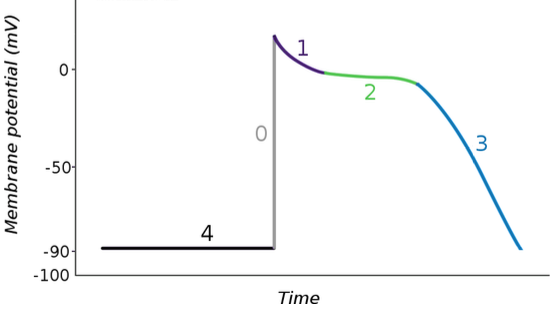
\includegraphics[width = 7cm]{./potential_cycle.png}
    \caption{Membrane potential in function of time (one cardiac cycle)}
    \label{potential_cycle}
    \end{center}
    \end{figure}
    
    \noindent The cell is initially at rest ($-90mV$, step 4). At a certain point, its potential increases rapidly ($\approx2ms$) and reaches the value of $+20mV$: the cell is activated. Later, a plateau near $0mV$ is observed and then a slow repolarization to the initial potential. \\
    From a microscopical point of view, we could study the dynamics acting in each single cell (as a consequence of the passage of chemical ions through specific channels, e.g. $Ca2+,Na+,K+$). From a macroscopical point of view, instead, one can observe it as a continuous electrical diffusion over the entire cardiac surface. Even if this consists in a very rapid phenomenon, the study of such propagation could be very interesting in order, for instance, to detect diseases in sick patients.
    
    \subsection{Mathematical models}
    Starting from the circuit in figure \ref{electrical_circuit}, applying some general electromagnetism laws and some calculations, the Bidomain model has been formulated (see \parencite{acta} for more details and/or \parencite{colli_franzone} for the complete passages).
    
    \begin{figure}[h]
    	\begin{center}
    		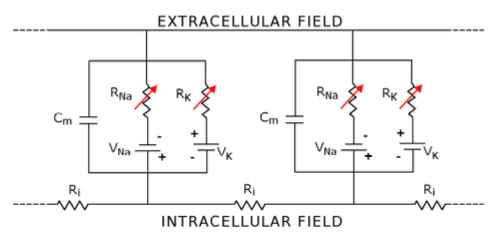
\includegraphics[width = 7cm]{./electrical_circuit.png}
    		\caption{Simplified circuit to model the intracellular and extracellular potentials dynamics}
    		\label{electrical_circuit}
    	\end{center}
    \end{figure}
    
    \noindent The general formulation is then: \vspace{3mm}
    \begin{definition}[Bidomain model]
	\begin{equation*}
	\begin{cases}
	\chi_m C_m\pdv{V_m}{t} - \nabla \cdot (\Sigma_i \nabla \phi_i) + \chi_m I_{ion} = I_i^{ext}    & \text{in } \Omega_{mus} \cross (0,T]
	\\
	-\chi_m C_m\pdv{V_m}{t} - \nabla \cdot (\Sigma_e \nabla \phi_e) - \chi_m I_{ion} = -I_e^{ext}    & \text{in } \Omega_{mus} \cross (0,T]
	\end{cases}
	\end{equation*}
    \end{definition}
	\vspace{3mm}
	
	where:
	\begin{itemize}[label=\textendash]
		\item $\bm{\phi_i, \phi_e}$ are the \emph{Intracellular and Extracelllular Potentials} (unknowns)
		\item $V_m = \phi_i-\phi_e$ is the \emph{Trans-membrane Potential}
		\item $\chi_m,C_m$ are known constants and $\Sigma_i, \Sigma_e$ are known constant tensors 
		\item $I_i^{ext},I_e^{ext}$ are applied currents
		\item $I_{ion}$ is the \emph{Ionic Current}
		\item $\Omega_{mus}$ is the cardiac domain (myocardium + endocardium + epicardium)
	\end{itemize}
    
    \vspace{4mm}
    \noindent Actually, this system is not complete since it misses boundary and initial conditions and a suitable model for $I_{ion}$. Initial conditions and Neumann boundary conditions for $\phi_i$ and $\phi_e$ are then imposed. For the definition of $I_{ion}$, instead, a \emph{reduced ionic model} is chosen, in particular the \emph{FitzHugh-Nagumo model}. Summing up:
    
    \begin{definition}[Bidomain + FitzHugh-Nagumo model with Neumann boundary conditions]\label{def1}
    	\begin{equation*}
    	\begin{cases}
    	\chi_m C_m\pdv{V_m}{t} - \nabla \cdot (\Sigma_i \nabla \phi_i) + \chi_m I_{ion}(V_m,w) = I_i^{ext}    & \text{in } \Omega_{mus} \cross (0,T]
    	\\
    	-\chi_m C_m\pdv{V_m}{t} - \nabla \cdot (\Sigma_e \nabla \phi_e) - \chi_m I_{ion}(V_m,w) = -I_e^{ext}    & \text{in } \Omega_{mus} \cross (0,T]
    	\\
    	I_{ion}(V_m,w)=kV_m(V_m-a)(V_m-1)+w & \text{in } \Omega_{mus} \cross (0,T]
    	\\
    	\pdv{w}{t} = \epsilon(V_m-\gamma w)  & \text{in } \Omega_{mus} \cross (0,T]
    	\\
    	\Sigma_i\nabla \phi_i \cdot n = b_i   & \text{on } \partial \Omega_{mus} \cross (0,T]
    	\\
    	\Sigma_e\nabla \phi_e \cdot n = b_e   & \text{on } \partial \Omega_{mus} \cross (0,T]
    	\\
    	\text{Initial conditions for } \phi_i,\phi_e, w & \text{in } \Omega_{mus}\cross\{t=0\}
    	\end{cases}
    	\end{equation*}
    \end{definition}
    \vspace{3mm}
    where:
    \begin{itemize}[label=\textendash]
    	\item $\bm{w}$ is the \emph{gating variable} (unknown)
    	\item $k,a,\epsilon,\gamma$ are known constants
    	\item $b_i,b_e$ are the boundary conditions data
    	\item $n$ is the outward normal vector
    \end{itemize}

    \vspace{4mm}
    \noindent From now on, the system of definition \ref{def1} will be the reference analytical problem for the development of numerical schemes.\\
    To conclude, there exist other famous and useful models, such as the \emph{Monodomain model}. But this is just a simplification of the Bidomain as in this case it is assumed that $\phi_i$ and $\phi_e$ are proportional. However, thanks to its simplicity, we often tested the code starting from the Monodomain implementation of the project \cite{andreotti} instead of analyzing directly the Bidomain.

    \subsection{A short discussion about the past works issue}
    As we have already introduced, our project initially aimed to continue and improve the work of a previous project (\parencite{marta}). \\
    Results obtained using unitary parameters, namely $\chi_m =\Sigma_i= \Sigma_e= C_m= k = \epsilon= \gamma= a=1$, were actually quite satisfactory. On the other hand, the choice of more realistic/experimental values for the parameters (that are often very big or very small) caused bad consequences to the accuracy of the schemes or even to their stability. In particular, we observed that the choice of $C_m \approx 10^{-2}$ highly compromised the stability of the numerical schemes.
    This issue heavily limits the use of the code for research and/or experimental simulations as it guarantees convergence to the right solution only in few and non-realistic problems.  \\

    \noindent After a while, we realized that an inverted sign of the FitzHugh-Nagumo model formula occurred in \cite{acta}. \\

    \noindent This oversight was not only essential for the fidelity to the real phenomena but also crucial for the well-posedness of the problem.\\ 
    We could give two motivations to reinforce this last statement: first of all, if we consider the well known study of \citeauthor{bourgault} (\cite{bourgault}), the conditions required for the well-posedness of the Bidomain problem are not satisfied if the sign is inverted (neither for the existence, hypothesis H4, nor for the uniqueness).\\ Secondly, suppose to discretize the Bidomain problem in time and to treat the non-linear term semi-implicitly, as it will be done in the following sections. Then, if we fix the timestep and if data from the previous timestep are given, we achieve a linear problem that can be easily switched into a weak formulation. From this analysis, we could observe that if $V_m<a$ or $V_m>1$ and $C_m$ is sufficiently small, the associated bilinear form is not coercive. \\

    \noindent This second motivation, even if not very formal and with a mixed approach, is particularly interesting since a few confirmations occurred during simulations, as shown for instance in figure \ref{sol_ill_posed}.


\begin{figure}[h]
	\begin{center}
		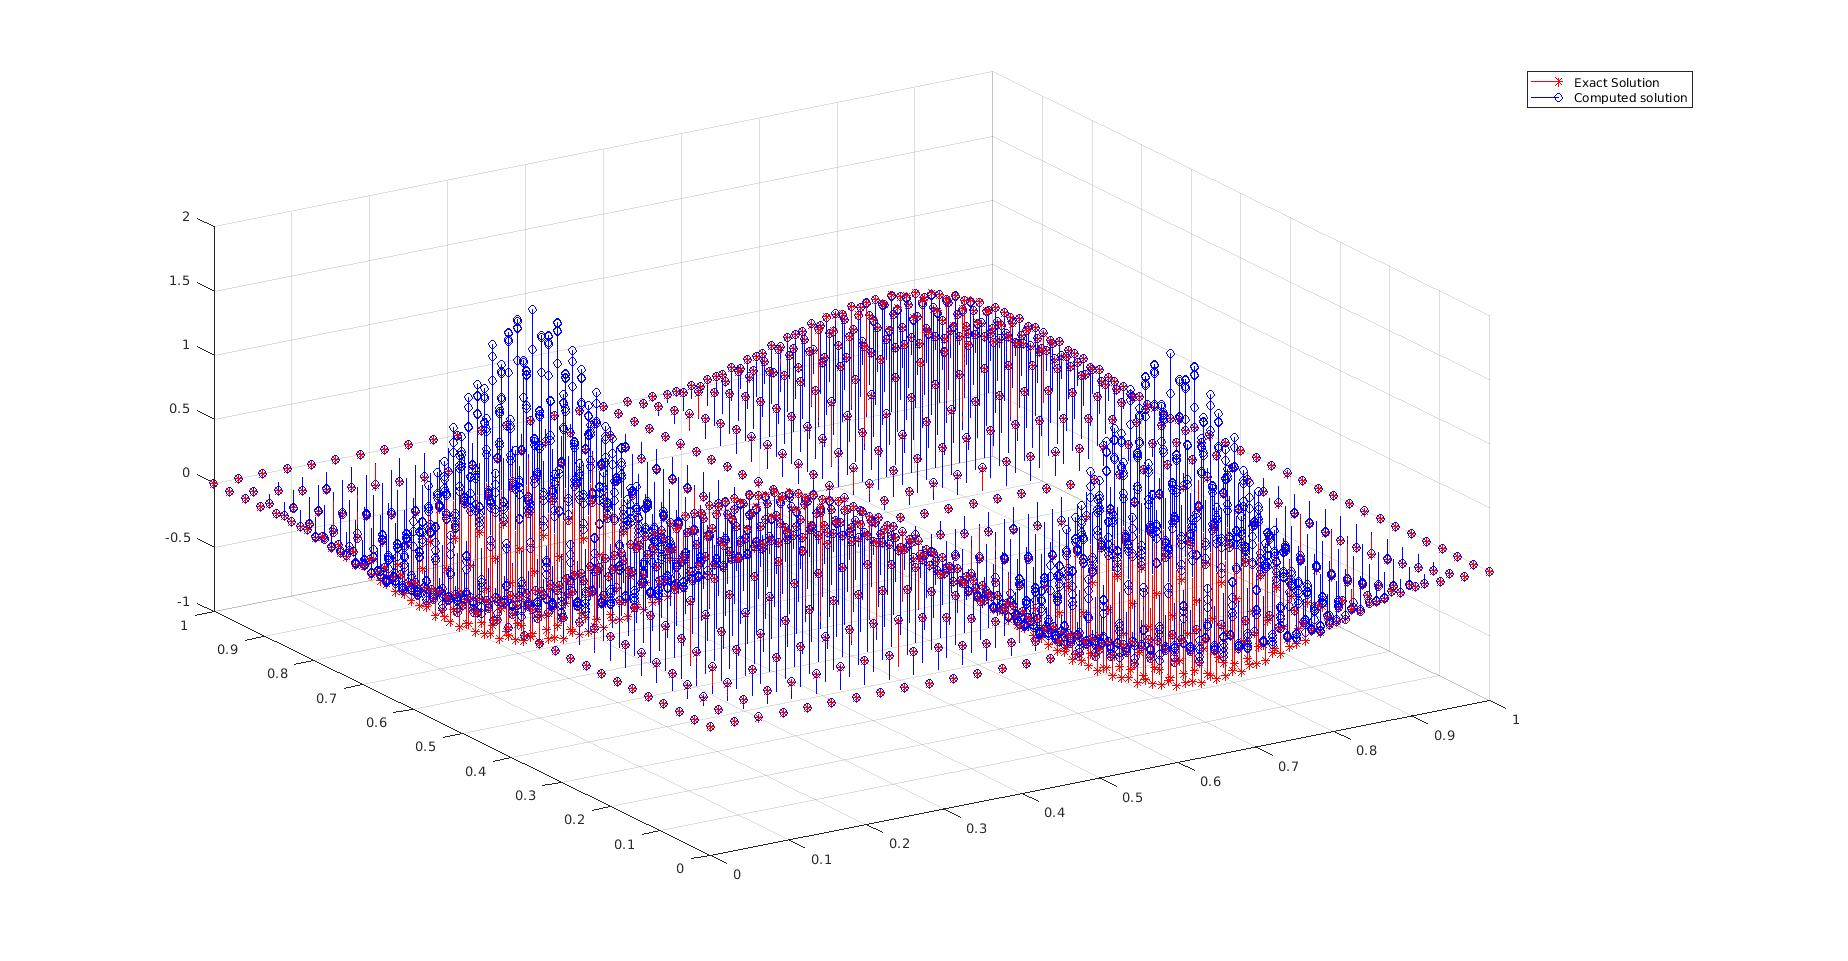
\includegraphics[width = 11cm]{./sol_ill_posed.jpg}
		\caption{Comparison between exact and computed solution with inverted FitzHugh-Nagumo model: huge errors arise only when $Vm<0$}
		\label{sol_ill_posed}
	\end{center}
\end{figure}
    
    \noindent In conclusion, the issue of the past works \cite{andreotti}, \cite{marta} had not a numerical nature as expected, but instead an analytical origin due to an ill-posed problem.



    \section{Semi discretized numerical methods}
    \subsection{DG discrete formulation}
    Starting from the strong form in definition \ref{def1}, the next step is the achievement of a suitable Discontinuous Galerkin weak formulation. Full descriptions and justifications of all the terms are present in \cite{marta} . \\
    Let us introduce a triangulation $\tau_h$ over $\Omega$, with $\mathcal{F} _h=\mathcal{F} _h^I \cup \mathcal{F} _h^B$ set of the faces of the elements, which includes the internal and boundary faces respectively, and the DG space $V_h^k = \{v_h \in L^2(\Omega) : v_h|_\mathcal{K} \in \mathbb{P}^{k}(\mathcal{K})  \quad \forall \mathcal{K} \in \tau_h \}$, where $k$ is the degree of the piecewise continuous polynomial. Moreover, we define $N_h=dim(V_h^k)<\infty$. \vspace{4mm}
    \begin{problem}[DG weak formulation]
    For any $t\in[0,T]$ find $\Phi_h(t)=[\phi_i^h(t),\phi_e^h(t)]^T \in [V_h^k]^2$  and  $w_h(t) \in V_h^k$ such that: \\
    \begin{enumerate}
    \item 
    \begin{equation*}
    \begin{gathered}
    \sum_{K \in \tau_h} \int_K{ \chi_m C_m \pdv{V_m^h}{t} V_h dw}+a_i(\phi_i^h,v_h)+\sum_{K \in \tau_h} \int_K{ \chi_m k (V_m^h-1)(V_m^h-a) V_m^h v_h dw}+\\
    +\sum_{K \in \tau_h} \int_K{ \chi_m w_h v_h dw}=(I_i^{ext},v_h) \qquad \forall v_h \in V_h^p\\
    \end{gathered}
    \end{equation*}
    \item
    \begin{equation*}
    \begin{gathered}
    -\sum_{K \in \tau_h} \int_K{ \chi_m C_m \pdv{V_m^h}{t} V_h dw}+a_e(\phi_e^h,v_h)-\sum_{K \in \tau_h} \int_K{ \chi_m k (V_m^h-1)(V_m^h-a) V_m^h v_h dw}+\\
    -\sum_{K \in \tau_h} \int_K{ \chi_m w_h v_h dw}=(-I_e^{ext},v_h) \qquad \forall v_h \in V_h^p\\
    \end{gathered}
    \end{equation*}
    \item
    \begin{equation*}
    \sum_{K \in \tau_h} \int_K{\pdv{w_h}{t}v_h dw}=\sum_{k \in \tau_h} \int_K{\epsilon (V_m^h-\gamma w_h) v_h dw} \qquad \forall v_h \in V_h^p\\
    \end{equation*}
    \end{enumerate}
    \vspace{5mm}
    where:
    \vspace{3mm}
    \begin{equation*}
    \begin{aligned}
    \bullet& \quad a_k(\phi_k^h,v_h)=\sum_{K \in \tau_h} \int_K{(\Sigma_k \nabla_h \phi_k^h) \cdot \nabla_h v_h dw}-\sum_{F \in \mathcal{F}_h^I} \int_F { \{\{\Sigma_k \nabla_h \phi_k^h \}\} \cdot [[v_h]] d\sigma}+\\
    &-\delta \sum_{F \in \mathcal{F}_h^I} \int_F{ \{\{\Sigma_k \nabla_h v_h\}\} \cdot [[\phi_k^h]]d\sigma}+\sum_{F \in \mathcal{F}_h^I}\int_F {\gamma [[\phi_k^h]] \cdot [[v_h]] d\sigma} \qquad k=i,e\\
    \newline
    \bullet& \quad (I_i^{ext},v_h)=\sum_{K \in \tau_h} \int_K {I_i^{ext} v_h dw}+\int_{\partial w}{b_i v_h d\sigma}\\
    \newline
    \bullet& \quad (-I_e^{ext},v_h)=-\sum_{K \in \tau_h} \int_K {I_e^{ext} v_h dw}+\int_{\partial w}{b_e v_h d\sigma}
    \end{aligned}
    \end{equation*}
    
    \noindent Moreover, according to the choice of the coefficient $\delta$, we can define:
    \begin{itemize}
    \item $\delta=1$: Symmetric Interior Penalty method (SIP)
    \item $\delta=0$: Incomplete Interior Penalty method (IIP)
    \item $\delta=-1$: Non Symmetric Interior Penalty method (NIP) 
    \end{itemize}
     \vspace{2mm}
    \noindent And $\gamma := \alpha \frac{k^2}{h}$ ("Stabilization parameter"),$ \quad \alpha \in \mathbb{R}$ to be chosen high enough.
    \end{problem}

    \vspace{4mm}
    \subsection{Algebraic formulation}
    Taking $\{\varphi_j\}_{j=1}^{N_h}$ base of $V_h^k$, so that we can write
    \begin{equation*}
    \begin{gathered}
    \Phi_h(t) = \begin{bmatrix} \phi_i^h(t) \\ \phi_e^h(t) \end{bmatrix} = \begin {bmatrix}\sum_{j=1}^{N_h} \phi_{i,j}(t)\varphi_j \\ \sum_{j=1}^{N_h} \phi_{e,j}(t)\varphi_j \end{bmatrix}\\
    w_h(t) = \sum_{j=1}^{N_h}w_j(t)\varphi_j\\
    V_m^h(t)=\sum_{j=1}^{N_h} V_{m,j}(t) \phi_j=\sum_{j=1}^{N_h}(\phi_{i,j}(t)-\phi_{e,j}(t))\varphi_j
 \end{gathered}
 \end{equation*}
 Then, we introduce the matrices:
 \begin{equation}\label{matrices}
\begin{rcases}
(V_k)_{ij} &= \int_{w}\nabla\varphi_j \cdot \Sigma_k \nabla \varphi_i 
\\ (I_k^T)_{ij} &= \sum_{F \in F_h^I} \int_{F} \{\{\Sigma_k \nabla\varphi_j\}\} \cdot [[\varphi_i]] 
\\ (I_k)_{i,j} &= \sum_{F \in F_h^I} \int_{F} [[\varphi_j]] \cdot \{\{\Sigma_k \nabla \varphi_i\}\}
\\(S_k)_{i,j} &= \sum_{F \in F_h^I} \int_{F} \gamma_k[[\varphi_j]] \cdot [[\varphi_i]]
\end{rcases}
\begin{gathered}
\quad A_k = (V_k -I_k^T - \theta I_k + S_k)\\
k=i,e \\
\end{gathered}
\end{equation}
\begin{equation*}
\gamma_k\vert_F = (n_F^T \, \Sigma_k \, n_F) \,\gamma, \quad n_F \text{ outward normal vector of F}
\end{equation*}

\begin{equation}
A_i \qquad{\text{Intra-cellular stiffness matrix}}
\end{equation}
\begin{equation}
A_e \qquad{\text{Extra-cellular stiffness matrix}}
\end{equation}
\begin{equation}
M_{ij} = \sum_{K \in \tau_h}\int_K\varphi_j\varphi_i \qquad{\text{Mass matrix}}
\end{equation}
\begin{equation}
C(u_h)_{ij} =  \sum_{K \in \tau_h} \int_K \chi_m k(u_h-1)(u_h-a)\varphi_j\varphi_i \qquad{\text{Non-linear matrix}}
\end{equation}
\begin{equation}
F_k=\begin{bmatrix} F_{i,k} \\ F_{e,k} \end{bmatrix}=\begin{bmatrix} \int_{w} I_i^{ext}\varphi_k - \sum_{F \in F_h^B} \int_F b_i\varphi_k \\ - \int_{w} I_e^{ext}\varphi_k - \sum_{F \in F_h^B} \int_F b_e\varphi_k \end{bmatrix}
\end{equation}
\vspace{3mm} \\
Therefore, our semi-discrete algebraic formulation is: \vspace{3mm}
\begin{problem}[DG algebraic formulation]\label{algebraic}
Find $\Phi_h(t)=[\phi_i^h(t),\phi_e^h(t)]^T \in [V_h^k]^2$ and $w_h(t) \in V_h^k$ for any $t \in (0;T]$ such that:
\begin{equation*}
\begin{cases}
\chi_m Cm M \dot{V_m^h}+A_i \phi_i^h+C(V_m^h) V_m^h+\chi_m M w_h=F_i^h \vspace{2mm} \\ 
-\chi_m Cm M \dot{V_m^h}+A_e \phi_e^h-C(V_m^h) V_m^h-\chi_m M w_h=F_e^h \vspace{2mm} \\ 
M \dot{w}_h(t)=\epsilon M (V_m^h(t)-\gamma w_h(t))
\end{cases}
\end{equation*}
\end{problem}
 \vspace{5mm}
 \noindent An alternative and more compact version with block matrices: \vspace{3mm}
 \begin{problem}[DG algebraic formulation - 2] \label{block_matrix}
 Find $\Phi_h(t)=[\phi_i^h(t),\phi_e^h(t)]^T \in [V_h^k]^2$ and $w_h(t) \in V_h^k$ for any $t \in (0;T]$ such that:
 \begin{enumerate}[label=\Roman*]
 \item
 \begin{equation*}
 \begin{gathered}
 \chi_mC_m \begin{bmatrix}M &-M \\ -M & M \end{bmatrix}
	\begin{bmatrix}\bm{\dot{\phi}_i^h(t)} \\ \bm{\dot{\phi}_e^h(t)} \end{bmatrix}
	 + \begin{bmatrix}A_i & 0 \\ 0 & A_e \end{bmatrix}
	 \begin{bmatrix}\bm{\phi_i^h(t)} \\ \bm{\phi_e^h(t)} \end{bmatrix} +\\
	   \begin{bmatrix}C(V_m^h) & -C(V_m^h) \\ -C(V_m^h) & C(V_m^h) \end{bmatrix} 
	   \begin{bmatrix} \bm{\phi_i^h(t)} \\ \bm{\phi_e^h(t)}  \end{bmatrix} 
	   +\chi_m \begin{bmatrix}M & 0 \\ 0 & -M \end{bmatrix} 
	   	\begin{bmatrix}w_h(t) \\ w_h(t) \end{bmatrix} = 
	   	\begin{bmatrix} F_i^h \\ F_e^h\end{bmatrix}
 \end{gathered}
 \end{equation*}
 \item
 \begin{equation*}
	   \dot{w}_h(t)=\epsilon (V_m^h(t)-\gamma w_h(t))
\end{equation*}
\end{enumerate}
\end{problem}
\vspace{5mm}
\section{Dubiner Basis}
    \subsection{Analytical aspects}\label{analytical_aspects}
    So far, we have described a general semi-discrete discontinuous formulation without examining which basis to use to generate the $V_h^k$ space. Usually, the common choice consists in the classical hat functions from FEM, even if they need to be modified in order to be used in a discontinuous context. It is also one of the simplest choices, for this reason our provided code was initially implemented with this basis. However, the very novelty of this study is the adoption of a new kind of basis, completely different from the previous and commonly known as "\emph{Dubiner Basis}" \cite{dubiner}. \\
    How we will soon see, the peculiarity of this family of functions is that it consists of orthogonal polynomials defined on the reference triangle
    \begin{equation}
    \hat{K}=\{ (\xi, \eta) : \xi, \eta \ge 0,	\xi+\eta \le 1 \}
    \end{equation}
    and not on the reference square
    \begin{equation}
    \quad \quad \hat{Q}=\{ (a, b) : -1 \le a \le 1, -1 \le b \le 1 \}
    \end{equation}
    Formally, if we consider the transformation from $\hat{Q}$ to $\hat{K}$
    \begin{equation}\label{transformation_formula}
    \xi:=\frac{(1+a)(1-b)}{4},  \eta:=\frac{(1+b)}{2}
    \end{equation}
    
    \begin{figure}[h]
    \begin{center}
    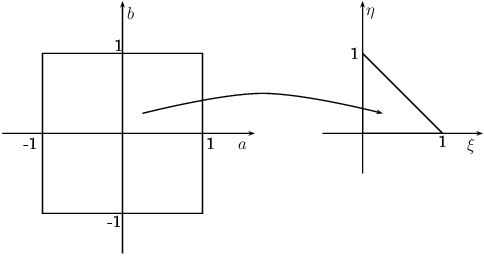
\includegraphics[width = 7cm]{./transformation.png}
    	\caption{Transformation between the reference square to the reference triangle}
    	\label{transformation}
    \end{center}
    \end{figure}
    
    \noindent the Dubiner basis is the transformation of a suitable basis initially defined on the reference square. This initial basis is simply obtained with a two dimensional modified tensor product of the Jacobi polynomials on the interval $(-1,1)$.
    \newpage
    \begin{definition}[Jacobi polynomials]
    The Jacobi polynomials of coefficients $\alpha,\beta \in \mathbb{R}$ evaluated in $z\in (-1,1)$ are:
    \begin{itemize}[label=\textendash]
    \item $n=0$
    \begin{equation}
    J_0^{\alpha,\beta}(z)=1
    \end{equation}
    \item $n=1$
    \begin{equation}
    J_1^{\alpha,\beta}(z)=\frac{1}{2}(\alpha-\beta+(\alpha+\beta+2)\cdot z);
    \end{equation}
    \item $n\ge2$
    \newline
    \begin{equation}
    \begin{gathered}
    \begin{aligned}
    J_n^{\alpha,\beta}(z)=\sum_{k=2}^{n} \Big[&\frac{(2k+\alpha+\beta-1)(\alpha^{2}-\beta^{2})}{2k(k+\alpha+\beta)(2k+\alpha+\beta-2)}+ \\ &\frac{(2k+\alpha+\beta-2)(2k+\alpha+\beta-1)(2k+\alpha \beta)}{2k(k+\alpha+\beta)(2k+\alpha+\beta-2)} J_{k-1}^{\alpha,\beta}(z) +
    \\-&\frac{2(k+\alpha-1)(k+\beta-1)(2k+\alpha+\beta)}{2k(k+\alpha+\beta)(2k+\alpha+\beta-2)} J_{k-2}^{\alpha,\beta}(z) \Big]
    \end{aligned}
    \end{gathered}
    \end{equation}
    \end{itemize}
    \end{definition}
    \vspace{5mm}
    \noindent An important property of these polynomials is:
    \begin{prop}
    $J_i^{\alpha,\beta}(\cdot)$ is orthogonal w.r.t. the Jacobi weight $w(x)=(1-x)^\alpha(1+x)^\beta$:
    \begin{equation}
    \int_{-1}^{1}{(1-x)^\alpha(1+x)^\beta J_m^{\alpha,\beta} J_q^{\alpha,\beta}(x)dx}=\frac{2}{2m+1} \delta_{mq} 
    \end{equation}
    \end{prop}
    
    \noindent Thanks to this definition, we can now define explicitly the Dubiner basis.
    \begin{definition}[Dubiner Basis] \label{dubiner}
    The Dubiner basis that generates the space $\mathbb{P}^p(\hat{K})$ of the polynomials of degree $p$ over the reference triangle is the set of functions:
    \begin{equation}
    \begin{split}
    \\
    & \quad \quad\quad  \quad \phi_{ij}: \hat{K} \rightarrow \mathbb{R} \\ \\
    \phi_{ij}(\xi,\eta) :&= c_{ij}(1-b)^j J_i^{0,0}(a) J_j^{2i+1,0}(b)=
    \\&=c_{ij} 2^j (1-\eta)^j J_i^{0,0}(\frac{2\xi}{1-\eta}-1) J_j^{2i+1,0} (2\eta-1) 
    \end{split}
    \end{equation}
    \vspace{3mm} \\
    for $i,j=1,\dots,p$ and $i+j \le p$, where
    \begin{equation}
    c_{ij} := \sqrt{\frac{2(2i+1)(i+j+1)}{4^i}}
    \end{equation}
    and $J_i^{\alpha,\beta}(\cdot)$ is the i-th Jacobi polynomial
    \end{definition}
    
    \vspace{5mm}
    \noindent As we have anticipated
    \begin{prop}\label{l2_ortho}
    The Dubiner basis is orthonormal in $L^2(\hat{K})$ $\forall p$:
    \begin{equation}
    \int_{\hat{K}}{\phi_{ij}(\xi,\eta)\phi_{mq}(\xi,\eta) d\xi d\eta}=\delta_{im}\delta_{jq}
    \end{equation}
    \end{prop}
    \vspace{4mm}
    \noindent As a consequence, after we successfully implemented the code with Dubiner basis and computed the matrices, we obtained a diagonal mass matrix (figure \ref{mass})
    
    \begin{figure}[ht]
    \begin{center}
    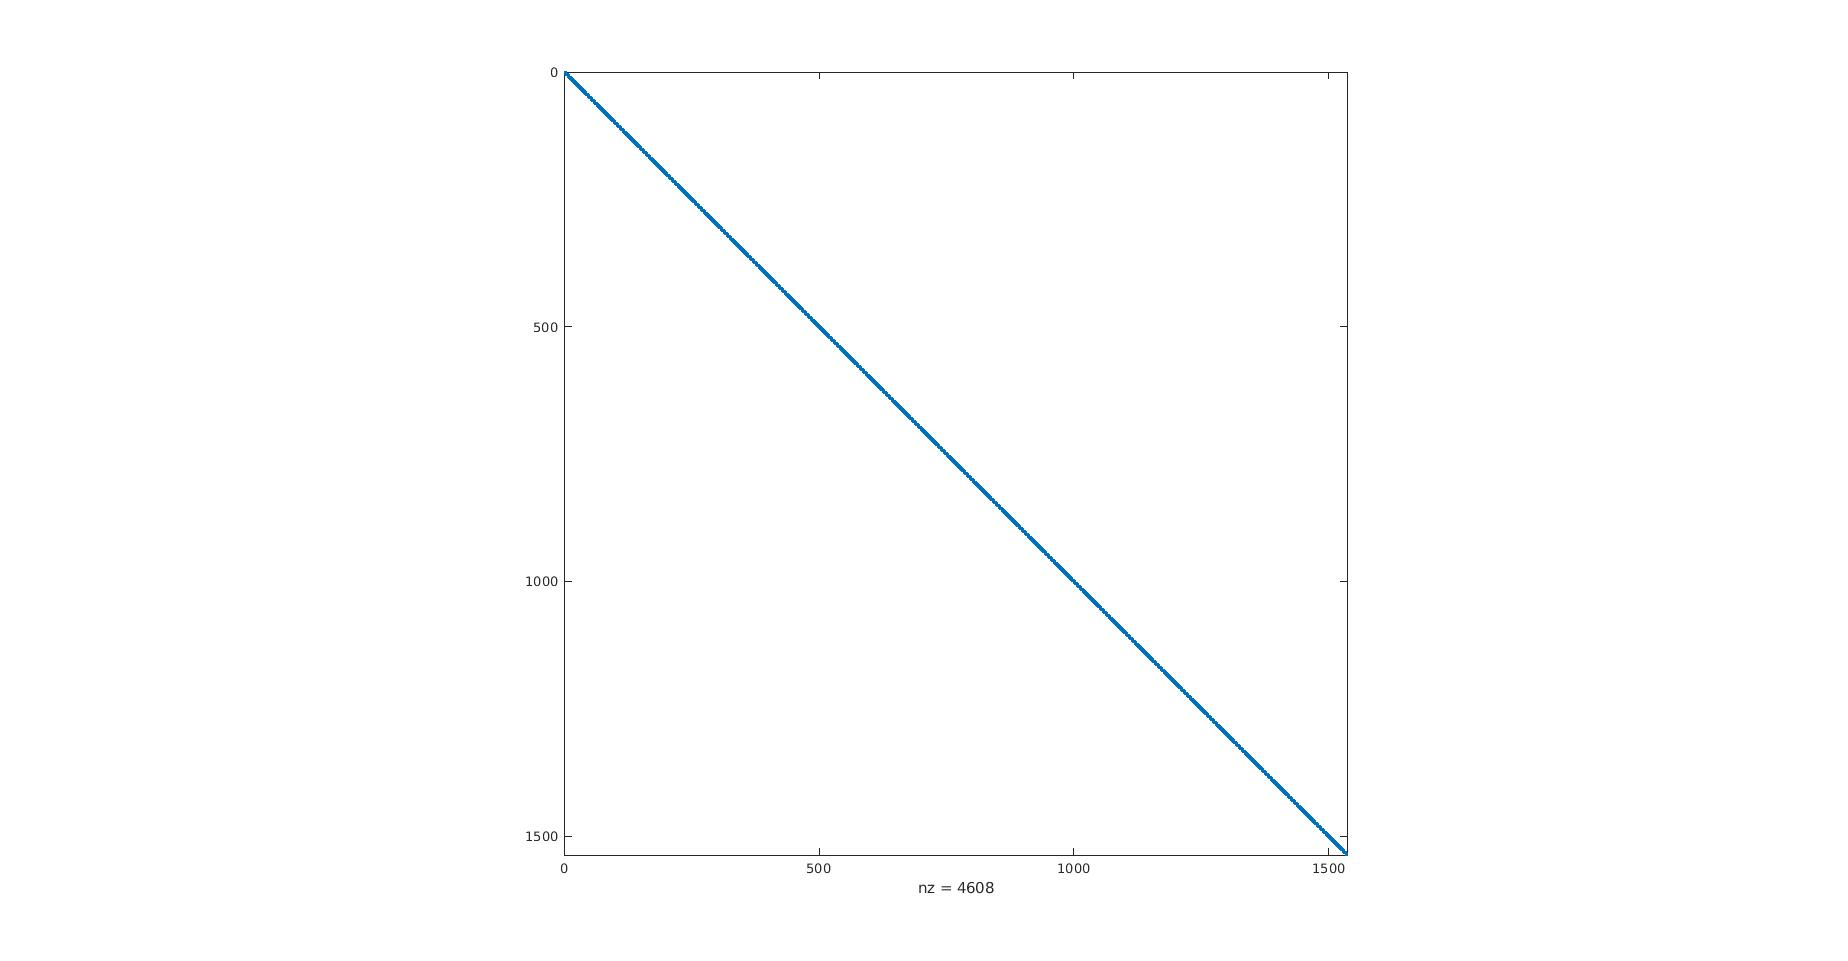
\includegraphics[width = 7cm]{./mass_dubiner.jpg}
    	\caption{Non-zero elements in the mass matrix when adopting Dubiner basis}
    	\label{mass}
    \end{center}
    \end{figure}

    \noindent It is noteworthy to point out that transformation \ref{transformation_formula} is bijective, it can be inverted but it needs some care. The natural inverse would be:
    
    \begin{equation}
    a = \frac{2\xi}{1-\eta}-1 \quad \quad b = 2\eta-1
    \end{equation}
    \vspace{2mm} \\
    \noindent that has already been used for the definition \ref{dubiner}. However, it is not defined for $\eta=1$, that means for the sole point $(0,1)$ of the reference triangle. To solve this issue, it is enough to prolong the function with continuity to this special point. For the code implementation, it is suggested avoiding evaluations in the exact point or adding an \emph{if} condition. We opted for the second solution. \\
    
    \noindent In general, the orthogonality property implies some good numerical properties, not only the diagonalization of the mass matrix. For instance, in \cite{antonietti} interesting bounds for the conditional number can be viewed. For this reason, we opted for this choice aiming to improve the previous results, at least from the space discretization side. \\
    
    \noindent On the other hand, there are also some difficulties arising when one chooses to abandon the familiar FEM basis. First of all, the coefficients of a discretized function has only \emph{modal} meaning and they no more represent the \emph{nodal} values of the function itself. This fact needs some extra work when one needs to switch from the continuous functions to the discretized functions and viceversa, as it will be shown in the paragraph \ref{subsection_implementation}. Secondly, one can notice that these functions are not boundary conditions friendly. What we mean is that, if compared to FEM basis, they have no particular properties on the boundary to let easily impose homogeneous boundary conditions. Thus, they should be again transformed, this time in a \emph{boundary adapted} form. We address to \cite{napde} for a short description of this procedure. Fortunately, we do not need to set this transformation as in the discontinuous formulation boundary conditions (both Dirichlet and Neumann) are imposed only weakly. It means that the boundary conditions' choice does not imply the choice of the vectorial space as in continuous Galerkin. The discretized space is always the same, only some terms in the weak formulation have in case of need to be changed. For this reason, the match of Discontinuous Galerkin and Dubiner Basis results to be particularly successful. \\
    
    \noindent To conclude, we refer to \cite{sherwin} for the transformation and the definition of the Dubiner Basis with tetrahedra, i.e. in dimension $n=3$.
    
    \subsection{Implementation}\label{subsection_implementation}
    Our code let the user to select which basis to adopt (FEM or Dubiner) and the order of polynomials until the order 3. We chose to call $D_1,D_2,D_3$ these 3 families of basis functions, thanks to the similarity to the $P_1,P_2,P_3$ finite element basis.\\
    The starting point was the implementation of some functions to evaluate the Dubiner basis functions and their gradients in the quadrature points. We omit the full code as it is not particular interesting: it barely follows the definitions of section \ref{analytical_aspects} with the addition of some technicalities. These mentioned scripts are: \texttt{eval\_jacobi\_polynomial.m}, \texttt{basis\_legendre\_dubiner.m}, \texttt{evalshape\_tria\_dubiner.m}.\\
    
    \noindent Moreover, some conditional statements and some extra methods (as the script \texttt{matrix2D\_dubiner.m}) were added to let the user easily switch from one basis to another (simply and once via \texttt{dati.m}). \\
    
    \noindent More interesting are instead the scripts \texttt{dubiner\_to\_fem.m} and \texttt{fem\_to\_dubiner.m}, used to convert the Dubiner modal coefficients of the vector solution to the nodal values of the approximated function and viceversa. For this reason, they deserve some further explanations.
\subsubsection{Switch from the modal coefficients to the nodal values}
One of the many advantages of the FEM basis is that there exists a bijection between the basis functions and some particular spacial points in such a way that the evaluation of a basis function in one of these points is equal to 1 only if that point is the one associated to the function, 0 otherwise:
	\begin{equation} \label{ref1}
	\psi_i(x_j)=\delta_{ij}
	\end{equation}
	Obviously, this property does not hold when we work with Dubiner basis. Indeed, these functions are not normalized on the mesh edges and they neither have an associated mesh point. This implies that the Dubiner coefficients of a function $u\in V_h^p$ are not the evaluation over these points of the discretized function itself. They have a completely different meaning, they are now \emph{modal} values instead of being \emph{nodal}.
	For this reason we introduced two new functions that best transform the coefficients of the solution w.r.t. FEM basis to the coefficients w.r.t. Dubiner basis and viceversa.\vspace{5mm}
	
	\noindent Consider an element $\mathcal{K}\in \tau_h$ and $\{\psi_{i}\}_{i=1}^{p}$,$\{\phi_{j}\}_{j=1}^{q}$ as, respectively, the set of FEM functions and the set of Dubiner functions with support in $\mathcal{K}$. In addition, consider as $\{\hat{u}_i\}_{i=1}^p$,$\{\tilde{u}_j\}_{j=1}^q$ as, respectively, the FEM and Dubiner coefficients of the solution. \vspace{5mm}
	
	\noindent Let us start from the transformation to the FEM coefficients. We now exploit the property \ref{ref1}, i.e. the coefficient $\hat{u}_i$ is nothing else but the evaluation of $u_h$ on the i-th mesh point, then: 
	\begin{equation} \label{ref3}
	\hat{u}_i = \sum_{j=1}^q \tilde{u}_j\phi_j(x_i)
	\end{equation}
	where $x_i$ is the point associated to the $\psi_i$ basis function. \vspace{5mm}
	
	\noindent Instead, to compute the coefficients conversely, we need to exploit the fact that the Dubiner Basis are $L^2$-orthonormal (proposition \ref{l2_ortho}). We then need to compute a $L^2$ scalar product between the FEM discretized function and each Dubiner basis function. That means:
	\begin{equation}\label{ref4}
	\tilde{u}_j = \int_\mathcal{K} u_h(x) \phi_j(x) \,dx = \int_{\mathcal{K}} \sum_{i=1}^p \hat{u}_i\psi_i(x) \phi_j(x) \,dx = \sum_{i=1}^p \Big(\int_{\mathcal{K}}\psi_i(x)\phi_j(x)\,dx \Big) \hat{u}_i
	\end{equation}
	
	\vspace{5mm}
	\noindent If the Dubiner functions are chosen as Galerkin basis, both the transformations are needed for the code implementation. Formula \ref{ref3} is needed to plot and compute errors after the resolution of the system (otherwise solely Dubiner coefficients are useless). Formula \ref{ref4} is instead needed to convert the FEM initial data $u_0$ into a vector of Dubiner coefficients before the resolution of the system.\\
	
	\noindent In order to be rigorous, but also for the sake of simplicity, these transformations are implemented only from $P_n$ to $D_n$, $n=1,2,3$ and viceversa. With this choice, the two basis generate the same space $V_h^n$ and then the transformation infers only on the coefficients and not on the function's properties. Otherwise, decreasing $n$ would mean to lose significant information, while increasing $n$ does not substantially improve the quality of the solution as it initially belonged to a lower order space. Moreover, choosing the same degree for P and D implies several semplifications, for instance the same number of local nodes ($nln$). For this reason, both $p$ and $q$ are actually replaced with $nln$ in the code.\\
	
	\noindent To conclude, formula \ref{ref3} to get nodal values has then been implemented in the following lines from the \texttt{dubiner\_to\_fem.m} script. 
	\begin{verbatim}
	function [u0] = dubiner_to_fem (uh, femregion, Data)  
	       
...
...
...

u0 = zeros(femregion.ndof,1);

% loop over all the elements
for ie = 1:femregion.ne
   
   % to get the global indexes for the nodes of ie 
   index = (ie-1)*femregion.nln*ones(femregion.nln,1) + [1:femregion.nln]';
   
   for i = 1 : femregion.nln
       for j = 1: femregion.nln
         u0(index(i)) = u0(index(i)) +  uh(index(j))*phi(1,i,j);
       end
   end
    
end
\end{verbatim}
\vspace{5mm}
\noindent On the other hand, the slightly more difficult formula \ref{ref4} have been reproduced in \texttt{fem\_to\_dubiner.m} using \emph{Gauss-Legendre-Lobatto} quadrature integration formulas. The main steps are the following:
\begin{verbatim}
function [u0] = fem_to_dubiner (uh, femregion, Data)

...
...
...

u0 = zeros(femregion.ndof,1);

% loop over all the elements
for ie = 1:femregion.ne

    % to get the global indexes for the nodes of ie 
    index = (ie-1)*femregion.nln*ones(femregion.nln,1) + [1:femregion.nln]';
    % loop over local degrees of freedom
    for i = 1 : femregion.nln
        % loop over 2D quadrature points
        for k = 1:length(w_2D) 
            uh_eval_k = 0;
            % loop to evaluate uh in a quadrature point
            for j = 1:femregion.nln
                uh_eval_k = uh_eval_k + uh(index(j))*phi_fem(1,k,j);
            end
            u0(index(i)) = u0(index(i)) + uh_eval_k*phi_dub(1,k,i).*w_2D(k);
        end
    end    
end
\end{verbatim}
\vspace{5mm}
\section{Temporal discretization}
So far, we have just studied the space discretization while a temporal discretization is still needed to totally discretize the Bidomain time-dependent problem. Thus, we divide the interval (0,T] into K subintervals $(t^k,t^k+1]$ of length $\Delta t$ such that $t^k=k \Delta t \quad \forall k=0,\cdots,K-1$, we then assume that $V_m^k\approx V_m(t^k)$. \\
We have developed, implemented and tested 3 different temporal strategies that we will refer to as: \emph{semi-implicit}, \emph{Godunov operator-splitting} and \emph{quasi-implicit operator-splitting}. 
\subsection{Semi-implicit method}
One of the most famous and used temporal scheme for a non-linear problem such as the Bidomain is certainly the \emph{Semi-Implicit} scheme \cite{acta}. The basic idea is to treat most of the terms implicitly while in fact treating the non-linear term semi-implicitly. Since the non-linear is cubic, the best choice is to treat only one of these $V_m$ terms implicitly, i.e.:
\begin{equation*}
I_{ion}^{k+1}=k(V_m^k-a)(V_m^k-1)V_m^{k+1}+w^{k+1}
\end{equation*}
at each time-step $k$ (different from the $k$ parameter). 
Moreover, the gating variable ODE is treated implicitly with the exception of the term $V_m$:
\begin{equation*}
M \frac{w^{k+1}-w^k}{\Delta t}=\epsilon M (V_m^k-\gamma w^{k+1})
\end{equation*}
\vspace{5mm} \\
Therefore, we can transform the semi-discrete problem \ref{block_matrix} into:
\begin{equation}
 \begin{gathered}
 \chi_mC_m \begin{bmatrix}M &-M \\ -M & M \end{bmatrix}
	\begin{bmatrix}\bm{\frac{\phi_i^{k+1}-\phi_i^{k}}{\Delta t}} \\ \bm{\frac{\phi_e^{k+1}-\phi_e^{k}}{\Delta t}}  \end{bmatrix}
	 + \begin{bmatrix}A_i & 0 \\ 0 & A_e \end{bmatrix}
	 \begin{bmatrix}\bm{\phi_i^{k+1}} \\ \bm{\phi_e^{k+1}} \end{bmatrix} +\\
	   \begin{bmatrix}C(V_m^h) & -C(V_m^h) \\ -C(V_m^h) & C(V_m^h) \end{bmatrix} 
	   \begin{bmatrix} \bm{\phi_i^{k+1}} \\ \bm{\phi_e^{k+1}}  \end{bmatrix} 
	   +\chi_m \begin{bmatrix}M & 0 \\ 0 & -M \end{bmatrix} 
	   	\begin{bmatrix}w^{k+1} \\ w^{k+1} \end{bmatrix} = 
	   	\begin{bmatrix} F_i^{k+1} \\ F_e^{k+1}\end{bmatrix}\\
	   M \frac{w^{k+1}-w^k}{\Delta t}=\epsilon M (V_m^k-\gamma w^{k+1})
\end{gathered}
\end{equation}\\
We remind that $V_m^k=\phi_i^k-\phi_e^k$. Separating known and unknown terms, we obtain: \vspace{3mm}
\begin{equation}
\begin{gathered}
\left( \frac{\chi_m C_m}{\Delta t} \begin{bmatrix} M & -M \\ -M & M \end{bmatrix} + \begin{bmatrix} A_i & 0 \\ 0 & A_e \end{bmatrix} + 
\begin{bmatrix}
C(V_m^k) & -C(V_m^k) \\ -C(V_m^k) & C(V_m^k)
\end{bmatrix}\right)
\begin{bmatrix} \bm{\phi_i^{k+1}} \\ \bm{\phi_e^{k+1}} \end{bmatrix} = 
\\
\begin{bmatrix} F_i^{k+1} \\ F_e^{k+1} \end{bmatrix} 
- \chi_m \begin{bmatrix}M & 0 \\ 0 & -M \end{bmatrix}
\begin{bmatrix} w^{k+1} \\ w^{k+1} \end{bmatrix}
+ \frac{\chi_m C_m}{\Delta t} \begin{bmatrix}M & 0 \\ 0 & -M\end{bmatrix}
\begin{bmatrix} V_m^{k} \\ V_m^{k} \end{bmatrix} \\
(\frac{1}{\Delta t}+\epsilon \gamma)M w^{k+1}=\epsilon M V_m^k+\frac{M}{\Delta t} w^k
\end{gathered}
\end{equation}

\vspace{5mm}
\noindent If we define:
\begin{itemize}
\item $B=\frac{\chi_m C_m}{\Delta t} \begin{bmatrix} M &-M \\-M & M \end{bmatrix}+\begin{bmatrix} A_i & 0 \\ 0 & A_e \end{bmatrix}$
\item $C_{nl}(V_m^k)=\begin{bmatrix}C(V_m^h) & -C(V_m^h) \\ -C(V_m^h) & C(V_m^h) \end{bmatrix}$
\item $r^{k+1}=\begin{bmatrix} F_i^{k+1} \\ F_e^{k+1}\end{bmatrix}-\chi_m \begin{bmatrix}M & 0 \\ 0 & -M \end{bmatrix} \begin{bmatrix}w^{k+1} \\ w^{k+1} \end{bmatrix}+\frac{\chi_m C_m}{\Delta t} \begin{bmatrix} M &-M \\-M & M \end{bmatrix} \begin{bmatrix} \phi_i^k \\ \phi_e^k \end{bmatrix}$
\end{itemize} \vspace{5mm}
we get the system in the final form: 
\begin{problem}[Semi-implicit discretized system]
Find $\Phi^{k+1}=[\phi_i^{k+1} \phi_e^{k+1}]^T$ and $w^{k+1}$ $\forall k=0,\cdots,T-1$ such that:
\begin{equation}
\begin{cases}
(\frac{1}{\Delta t}+\epsilon \gamma)M w^{k+1}=\epsilon M V_m^k+\frac{M}{\Delta t} w^k \\
(B+C_{nl}(\Phi^k)) \Phi^{k+1}=r^{k+1}
\end{cases}
\end{equation} 
\end{problem}

\subsubsection{Implementation}
\begin{verbatim}
MASS = [M -M; -M M];
ZERO = sparse(length(M), length(M));
MASS_W = [M ZERO; ZERO -M];
STIFFNESS = [Ai ZERO; ZERO  Ae];

for t=dt:dt:T

   w1 = 1/(1+epsilon*gamma*dt)*(w0+epsilon*dt*Vm0);
   w1=cat(1,w1, w1);
   Vm0 = cat(1,Vm0,Vm0);

   fi = assemble_rhs_i(femregion,neighbour,Data,t);
   fe = assemble_rhs_e(femregion,neighbour,Data,t);
   f1 = cat(1, fi, fe);

   [C] = assemble_nonlinear(femregion,Data,Vm0);
   NONLIN = [C -C; -C C];

   r = f1 + ChiM*Cm/dt * MASS_W * Vm0 - ChiM * MASS_W *w1;

   B=ChiM*Cm/dt * MASS + (STIFFNESS + NONLIN);

   u1 = B \ r;

   f0 = f1;
   Vm0 = u1(1:ll)-u1(ll+1:end);
   u0 = u1;
   w0 = w1(1:ll);
end
\end{verbatim}
\vspace{4mm}
\subsection{Godunov operator-splitting}
The main feature of a general operator-splitting method is the division of the problem into two different problems to be solved sequentially. This is possible and justified when the original functional operator $L$ is splitted into 2 different operators such that $L(u)=L_1(u)+L_2(u)$.
Two operator-splitting methods have been implemented, the first is of \emph{Godunov} type and a detailed study together with its properties can be found in \cite{spiteri}. The formulation is: \\ \\
\begin{center}Find $\hat{V}_m^{k+1},\phi_i^{k+1},\phi_e^{k+1},w^{k+1}$ such that:\end{center}
\begin{enumerate}[label = \Roman*]
\item
\begin{equation*}
\begin{cases}
\chi_m C_m M\frac{\hat{V}_m^{k+1} - V_m^k}{\Delta t} + C(V_m^k)V_m^k +\chi_mMw^k = 0\\
\frac{w^{k+1}-w^k}{\Delta t} = \epsilon (V_m^k - \gamma w^k)
\end{cases}
\end{equation*}
\item
\begin{equation*}
\begin{cases}
\chi_m C_m M\frac{V_m^{k+1} - \hat{V}_m^{k+1}}{\Delta t} + A_i\phi_i^{k+1} = F_i^{k+1} \\
-\chi_m C_m M\frac{V_m^{k+1} - \hat{V}_m^{k+1}}{\Delta t} + A_e\phi_e^{k+1} = F_e^{k+1}
\end{cases}
\end{equation*}
\end{enumerate}
\noindent Putting in a unique system:
\begin{equation}\label{Godunov}
\begin{cases}
\chi_m C_m M\frac{V_m^{k+1} - V_m^k}{\Delta t} + C(V_m^k)V_m^k +\chi_mMw^k + A_i \phi_i^{k+1}= F_i^{k+1} \\
\chi_m C_m M\frac{V_m^{k+1} - V_m^k}{\Delta t} + C(V_m^k)V_m^k +\chi_mMw^k - A_e \Phi_e^{k+1}= -F_e^{k+1} \\
w^{k+1} = (1-\epsilon \gamma \Delta t) w^k + \epsilon \Delta t V_m^k
\end{cases}
\end{equation}
The equations in the system \ref{Godunov} can be rewritten as:
\begin{equation*}
\begin{cases}
\left( \frac{\chi_m C_m}{\Delta t} M + A_i \right ) \phi_i^{k+1} - \frac{\chi_m C_m}{\Delta t} M \phi_e^{k+1} = F_i^{k+1} - \chi_m M w^k + \left( \frac{\chi_m C_m}{\Delta t} M- C(V_m^k)\right) V_m^k\\
\frac{\chi_m C_m}{\Delta t} M  \phi_i^{n+1} - \left(\frac{\chi_m C_m}{\Delta t} M + A_e \right) \phi_e^{k+1} =  -F_e^{k+1} - \chi_m M w^k + \left( \frac{\chi_m C_m}{\Delta t} M- C(V_m^k)\right) V_m^k \\
w^{k+1} = (1-\epsilon \gamma \Delta t) w^k + \epsilon \Delta tV_m^k
\end{cases}
\end{equation*}

\noindent And then, we obtain the final form:
\begin{problem}[Godunov operator-splitting discretized system] 
	Find $\Phi^{k+1}=[\phi_i^{k+1} \phi_e^{k+1}]^T$ and $w^{k+1} \quad \forall k=0, \cdots, K-1$ such that: 
\begin{equation}
\begin{cases}
\begin{gathered}
\left(
\frac{\chi_m C_m}{\Delta t} \begin{bmatrix}M & -M \\ M & -M\end{bmatrix}
+ \begin{bmatrix} A_i & 0 \\ 0 & -A_e \end{bmatrix}
\right) \begin{bmatrix} \bm{\phi_i^{k+1}} \\ \bm{\phi_e^{k+1}}  \end{bmatrix} =
\begin{bmatrix} F_i^{k+1} \\ -F_e^{k+1} \end{bmatrix} + \\ -
\chi_m\begin{bmatrix} M & 0 \\ 0 & M \end{bmatrix} \begin{bmatrix} w^k \\ w^k \end{bmatrix} +
\left(\frac{\chi_mC_m}{\Delta t}\begin{bmatrix} M & 0 \\ 0 & M \end{bmatrix}
- \begin{bmatrix} C(V_m^k) & 0 \\ 0 & C(V_m^k)\end{bmatrix} 
\right) \begin{bmatrix} V_m^k \\ V_m^k \end {bmatrix}
\end{gathered} \\ \\
w^{k+1} = (1-\epsilon \gamma \Delta t) w^k + \epsilon \Delta tV_m^k
\end{cases}
\end{equation}
\end{problem}

\subsubsection{Implementation}
\begin{verbatim}
ZERO = sparse(ll,ll);
MASS = (ChiM*Cm/dt)*[M, -M; M -M];
MASSW = ChiM*[M, ZERO; ZERO, M];

for t=dt:dt:T

   fi = assemble_rhs_i(femregion,neighbour,Data,t);
   fe = assemble_rhs_e(femregion,neighbour,Data,t);
   f1 = cat(1, fi, -fe);

   [C] = assemble_nonlinear(femregion,Data,Vm0);

   w1 = (1 -epsilon*gamma*dt)*w0 + epsilon*dt*Vm0;
   B = MASS + [Ai, ZERO; ZERO, -Ae];
   r = -MASSW*[w0;w0] + ((Cm/dt)*MASSW - [C, ZERO; ZERO, C])
   *[Vm0;Vm0] + f1;

   Vm0 = u1(1:ll) - u1(ll+1:end);
   u0 = u1;
   w0 = w1;
end
\end{verbatim}
\vspace{4mm}
\subsection{Quasi-implicit operator-splitting}
The aim of a quasi-implicit operator splitting is to treat implicitly all the terms except the cubic one. Even if it cannot be defined as a full implicit method, we hope to achieve more stability if compared to the previous Godunov-kind scheme. This time, the formulation turns to be: \newline

\begin{center} Find $\tilde{V}_m^{k+1}, \phi_i^{k+1}, \phi_e^{k+1},w^{k+1}$ such that: \end{center}
\begin{enumerate}[label = \Roman*]
\item
\begin{equation*}
\begin{cases}
\chi_m C_m M \frac{\tilde{V}_m^{k+1}-V_m^k}{\Delta t} +  C(V_m^k) V_m^{k+1} + \chi_m M w^{k+1}= 0\\
\frac{w^{k+1} - w^k}{\Delta t} = \epsilon (V_m^{k+1}-\gamma w^{k+1})
\end{cases}
\end{equation*}
\item
\begin{equation*}
\begin{cases}
\chi_m C_m M \frac{V_m^{k+1}-\tilde{V}_m^{k+1}}{\Delta t} + A_i \phi_i^{k+1}= F_i^{k+1}\\
- \chi_m C_m M \frac{V_m^{k+1}-\tilde{V}_m^{k+1}}{\Delta t} + A_e \phi_e^{k+1}= F_e^{k+1}
\end{cases}
\end{equation*}
\end{enumerate}
\vspace{3mm}
Putting into a unique system:
\begin{equation}\label{Quasi}
\begin{cases}
\chi_m C_m M \frac{V_m^{k+1}-V_m^{k}}{\Delta t} + C(V_m^k) V_m^{k+1} + \chi_m M w^{k+1} + A_i \phi_i ^{k+1} = F_i^{k+1} \\
\chi_m C_m M \frac{V_m^{k+1}-V_m^{k}}{\Delta t} +  C(V_m^k) V_m^{k+1} + \chi_m M w^{k+1} - A_e \phi_e ^{k+1} =  -F_e^{k+1} \\
\frac{w^{k+1}-w^{k}}{\Delta t} = \epsilon(V_m^{k+1}-\gamma w^{k+1})
\end{cases}
\end{equation} 
\vspace{14mm} \\
If we define:
\begin{itemize}
\item $Q_k = \frac{\chi_m C_m}{\Delta t}M + C(V_m^k) + \frac{\epsilon\chi_m \Delta t}{1 + \epsilon \gamma \Delta t} M$ 
\item $R_k = \frac{\chi_mC_m}{\Delta t}MV_m^k - \frac{\chi_m}{1+\epsilon\gamma\Delta t}M w^k$
\end{itemize}
\vspace{4mm}
the equations in system \ref{Quasi} can be written as:
\begin{enumerate}
\item
\begin{equation*}
\begin{gathered}
\chi_m C_m M \frac{	\phi_i^{k+1}-\phi_e^{k+1}-V_m^{k}}{\Delta t} +  C(V_m^k) (\phi_i^{k+1}-\phi_e^{k+1}) + \chi_m M \left(\frac{w^k + \epsilon \Delta t (\phi_i^{k+1}-\phi_e^{k+1})}{1+\epsilon \gamma \Delta t}   \right)+\\
+ A_i \phi_i ^{k+1} = F_i^{k+1} \\
\Rightarrow \quad (Q_k + A_i) \phi_i^{k+1} - Q_k \phi_e^{k+1} =R_k +  F_i^{k+1}
\end{gathered}
\end{equation*}
\item
\begin{equation*}
\begin{gathered}
\chi_m C_m M \frac{	\phi_i^{k+1}-\phi_e^{k+1}-V_m^{k}}{\Delta t} + \cdot C(V_m^k) (\phi_i^{k+1}-\phi_e^{k+1}) + \chi_m M \left(\frac{w^k + \epsilon \Delta t (\phi_i^{k+1}-\phi_e^{k+1})}{1+\epsilon \gamma \Delta t}   \right) +\\
- A_e \phi_e ^{k+1} = -F_e^{k+1} \\ \\
\Rightarrow \quad Q_k \phi_i^{k+1} - (Q_k+A_e) \phi_e^{k+1} =R_k - F_e^{k+1}
\end{gathered}
\end{equation*}
\item 
\begin{equation*}
w^{k+1} = \frac{w^k + \epsilon \Delta t (\phi_i^{k+1}-\phi_e^{k+1})}{1+\epsilon \gamma \Delta t}
\end{equation*}
\end{enumerate}
\vspace{4mm}
The final system becomes:
\begin{problem} [Quasi-implicit operator-splitting discretized system]
Find $\Phi^{k+1}=[\phi_i^{k+1} \phi_e^{k+1}]^T$ and $w^{k+1} \quad \forall k=0, \cdots, K-1$ such that:
\begin{equation}
\quad
\begin{cases}
\left(
\begin{bmatrix} Q_k & -Q_k \\ Q_k & -Q_k \end{bmatrix} + 
\begin{bmatrix} A_i & 0 \\ 0 & -A_e\end{bmatrix}
\right)
\begin{bmatrix}
\bm{\phi_i^{k+1}} \\ \bm{\phi_e^{k+1}}
\end{bmatrix}
= \begin{bmatrix} R_k \\ R_k \end{bmatrix} + \begin{bmatrix} F_i^{k+1} \\  -F_e^{k+1}\end{bmatrix} \\ \\
w^{k+1} = \frac{\displaystyle w^k + \epsilon \Delta t (\phi_i^{k+1}-\phi_e^{k+1})}{\displaystyle 1+\epsilon \gamma \Delta t}
\end{cases}
\end{equation}
\end{problem}

\subsubsection{Implementation}
\begin{verbatim}
ZERO = sparse(ll,ll);
        
for t=dt:dt:T
        
   [C] = assemble_nonlinear(femregion,Data,Vm0);
   Q  = (ChiM*Cm/dt)*M + C - (epsilon*ChiM*dt)/(1+epsilon*gamma*dt)*M;
   R  = (ChiM*Cm/dt)*M*Vm0 - (ChiM)/(1+epsilon*gamma*dt)*M*w0;
    
   fi = assemble_rhs_i(femregion,neighbour,Data,t);
   fe = assemble_rhs_e(femregion,neighbour,Data,t);
   f1 = cat(1, fi, -fe);
    
   B = [Q, -Q; Q, -Q] + [Ai, ZERO; ZERO, -Ae];
   r = [R;R] + f1;
        
   u1 = B \ r; 
        
   Vm1 = u1(1:ll)-u1(ll+1:end);

   w1 = (w0 + epsilon*dt*Vm1)/(1+epsilon*gamma*dt);
    
   f0 = f1;
   Vm0 = u1(1:ll) - u1(ll+1:end);
   u0 = u1;
   w0 = w1;
end
\end{verbatim}

\section{About the potentials uniqueness}
\noindent Observing for a moment the Bidomain problem analytical formulation (definition \ref{def1}), we can immediately realize that the intracellular and the extracellular potentials appear only through their difference $V_m$ or their gradient. This means that there cannot be uniqueness for the two functions. Namely: \vspace{2mm}
\begin{equation}\label{phi_uniqueness}
\begin{gathered}
\phi_i,\phi_e \text{ classical solutions of Bidomain} \Rightarrow \phi_i+\varphi,\,\phi_e+\varphi \text{ are solutions as well } \\
 \forall \varphi: [0,T] \rightarrow \mathbb{R} \quad \text{ sufficiently regular}
\end{gathered}
\end{equation}

\vspace{4mm}
\noindent However, this fact should not surprise nor confuse the reader. First of all, we remind again that in \cite{bourgault} and \cite{colli_franzone} there are proofs for the $V_m$ and $w$ uniqueness, then this is taken for granted. Secondly, this statement reflects the physical intuition of the problem: cellular dynamics is not involved by potentials exact values but instead from their difference, in addition a potential value is nonsense if a convention value to compare it with has not been set. The dependence on time can be interpreted as follows: if, at any time instant, we change the conventional potential value, the dynamics of the problem does not change. \\

\noindent Moreover, we can give this simple result to show that the solutions of the form of equation \ref{phi_uniqueness} are also the only admissible:\\
\begin{theo}
	For the Bidomain problem coupled with Fitzhugh-Nagumo model with Neumann boundary conditions (definition \ref{def1}), the $\phi_i,\phi_e$ solutions are unique minus a constant depending only on time. 
\end{theo}

\begin{proof}
	\vspace{2mm} We remind that existence and uniqueness for $V_m$ and $w$ have already been proved in \cite{bourgault}. 
	Suppose now there exist two couples $(\phi_i^1,\phi_e^1)$,$(\phi_i^2,\phi_e^2)$ of potentials solutions of the Bidomain problem. If $V_m$ uniqueness holds, there must exist a unique value of $V_m$ such that:
	\begin{equation*}
	\phi_i^1-\phi_e^1 = \phi_i^2-\phi_e^2 = V_m
	\end{equation*}\\
	Then, we define a function $\varphi:\Omega \cross [0,T] \rightarrow \mathbb{R}$ as:
	\begin{equation*}
	\varphi := \phi_i^1-\phi_i^2 = \phi_e^1-\phi_e^2
	\end{equation*}\\
	If we consider the starting problem in definition \ref{def1}, the following equations must hold:
	\begin{equation*}
	\begin{cases}
	\chi_m C_m\pdv{V_m}{t} - \nabla \cdot (\Sigma_i \nabla \phi_i^1) + \chi_m I_{ion}(V_m,w) = I_i^{ext}    & \text{in } \Omega_{mus} \cross (0,T]
	\\
	\chi_m C_m\pdv{V_m}{t} - \nabla \cdot (\Sigma_i \nabla \phi_i^2) + \chi_m I_{ion}(V_m,w) = I_i^{ext}    & \text{in } \Omega_{mus} \cross (0,T]
	\\
	\Sigma_i\nabla \phi_i^1 \cdot n = b_i   & \text{on } \partial \Omega_{mus} \cross (0,T]
	\\
	\Sigma_i\nabla \phi_i^2 \cdot n = b_i   & \text{on } \partial \Omega_{mus} \cross (0,T]
	\end{cases}
	\end{equation*}\\
	Subtracting:
	\begin{equation*}
	\begin{cases}
	- \nabla \cdot (\Sigma_i \nabla \varphi) = 0    & \text{in } \Omega_{mus} \cross (0,T]
	\\
	\Sigma_i\nabla \varphi \cdot n = 0   & \text{on } \partial \Omega_{mus} \cross (0,T]
	\end{cases}
	\end{equation*} \\
	That is a classical \emph{Laplace problem} with homogeneous Neumann boundary conditions. From theory \cite{salsa}, we know that the solution is represented by all constant terms. However, we must pay attention to the fact that $\varphi$ is a time-dependent function, even if time does not compare in the system. Thus, we can state:
	
	\begin{equation*}
	\exists \tilde{\varphi}:[0,T]\rightarrow \mathbb{R} \text{ such that } \varphi(x,t) = \tilde{\varphi}(t) \quad \forall x \in \Omega,\forall t \in [0,T] 
	\end{equation*}\\
	To conclude, we can observe now that if these two couples of solutions exist, then:
	\begin{equation*}
	\phi_i^1-\phi_i^2 = \phi_e^1-\phi_e^2=\tilde{\varphi} \quad \forall x \in \Omega, \forall t \in [0,T]
	\end{equation*}
\end{proof}

\begin{remark}
For what concerns the regularity of $\varphi$, we can certainly state that, as a difference of two sufficiently regular functions, it belongs to the same class of regularity of the potentials if restricted to the sole time variable.
\end{remark}

\vspace{4mm}
\noindent We can conclude this analytical digression with an accomplished necessary and sufficient condition for the potentials solutions. \vspace{4mm}

\begin{corollary}
Suppose the couple ($\phi_i,\phi_e$) is a classical solution of the problem of definition \ref{def1} (for a certain $w$). The couple ($\tilde{\phi}_i,\tilde{\phi}_e$) of sufficiently regular real functions defined in $\Omega\cross[0,T]$ is another couple solution if and only if both $\tilde{\phi}_i,\tilde{\phi}_e$ differ respectively from $\phi_i,\phi_e$ for a time-dependent function $\varphi$ that belongs to the union of the regularity classes of the previous functions if restricted to time variable.
\end{corollary}

\begin{proof}
	The regularity statement is trivial and already discussed. The right implication is due to the previous theorem. Finally, the left implication follows what has been shown in equation \ref{phi_uniqueness}: it is enough to insert $\phi_i+\varphi$ and $\phi_e+\varphi$ in the Bidomain system to find out that $\varphi$ disappears and the remaining system is the same as the one with $\phi_i,\phi_e$, thus solved by hypothesis.
\end{proof}
	

    \newpage
    \printbibliography

\end{document}

    
	
    
    
    
    
    
    
    
    
    
    
    
    \newpage
    \printbibliography

\end{document}
